\documentclass{article}

\usepackage[english]{babel}
\usepackage{fancyhdr}
% Make tables work proper 
% \usepackage{amstext} % for \text macro
% \usepackage{array}   % for \newcolumntype macro
% \newcolumntype{L}{>{$}r<{$}} % math-mode version of "l" column type
% \newcolumntype{R}{>{$}r<{$}} % math-mode version of "r" column type
 
% Write proper math 
\usepackage{amssymb}

% URLS 
\usepackage{hyperref}

% Reference smart
\usepackage{cleveref}

% Font modifiers
\usepackage[utf8]{inputenc}
\usepackage[T1]{fontenc}
\usepackage{fontspec}

% update to modern math font
\usepackage{cmbright}

% titlesec allows us to redefine our headings
\usepackage{titlesec}

% include quotes 
\usepackage{csquotes}
\usepackage{color, soul}

% graphicx for graphics 
\usepackage{tikz}
\usepackage{graphicx}
\graphicspath{ {./gfx/} }

% formatting geometry and paper stuff
\usepackage[
    paper=a4paper,
    % showframe, % debugging
    margin=1.5in]{geometry}% http://ctan.org/pkg/geometry


% !! TESTING 

% \usepackage{blindtext}



%% FONTS SPECIFIED HERE: USE ONE OF THE TWO:

% %% USE PRIMARY FONTS: 
% \setsansfont[
% Extension = .otf ,
% Path=./fnt/primary/ ,
% UprightFont=*-Regular,
% ItalicFont=*-RegularItalic,
% BoldFont=*-Bold,
% BoldItalicFont=*-BoldItalic,
% ]{MessinaSans}

% \setmainfont[
% Extension = .otf ,
% Path=./fnt/primary/ ,
% UprightFont=*-Regular,
% ]{Nantes}


%% USE SECONDARY FONTS (open source): 
% \setsansfont[
% Extension = .ttf ,
% Path=./fnt/secondary/Roboto/ ,
% UprightFont=*-Regular,
% BoldFont=*-Bold,
% ItalicFont=*-Italic,
% BoldItalicFont=*-BoldItalic,
% ]{Roboto}

\setsansfont[
Extension = .ttf ,
Path=./fnt/secondary/Inter/ ,
UprightFont=*-Light,
BoldFont=*-SemiBold,
% BoldFont=*-Regular,
]{Inter}

\setmainfont[
Extension = .otf ,
Path=./fnt/secondary/Noto_Serif_SC/ ,
UprightFont=*-Regular,
BoldFont=*-Bold,
% ItalicFont=*-Italic,
% BoldItalicFont=*-BoldItalic,
]{NotoSerifSC}



% Roboto mono as universal 
\setmonofont[
Extension = .ttf ,
Path=./fnt/ ,
UprightFont=*-Light,
BoldFont=*-Regular,
]{RobotoMono}





% section titles in serif
% \titleformat{\section}{\HUGE\mdseries\rmfamily\leftalign}
% \titleformat{\subsection}{\LARGE\mdseries\rmfamily}
% \titleformat{\subsubsection}{\large\mdseries\rmfamily}
% switch between bfseries and mdseries to get bold face or not
\titleformat*{\section}{\huge\mdseries\rmfamily}
\titleformat*{\subsection}{\Large\mdseries\rmfamily}
\titleformat*{\subsubsection}{\large\mdseries\rmfamily}
\titleformat*{\paragraph}{\normalsize\bfseries\rmfamily} 

% Set main font to be sans serif 
\renewcommand{\familydefault}{\sfdefault}

% PAGE STYLE HEADER AND FOOTER
\setlength{\headheight}{30pt} 
\pagestyle{fancy}
\fancyhf{}
\fancyhead[RE,LO]{ 
\includegraphics[height=30pt]{logo/Corti-Symbol-Black-CMYK.pdf}  }
\fancyhead[LE,RO]{\leftmark}
\cfoot{\thepage}
% \fancyfoot[LE,RO]{\thepage}
% \fancyfoot[LE,RO]{\thepage}



% Start counting sections at 0 
\setcounter{section}{-1}

%%%%%%%%%%%%%%%%%
% Document here %
%%%%%%%%%%%%%%%%%
\begin{document}

\setcounter{page}{0}
\begin{titlepage}
\newgeometry{top=1in,bottom=1in,right=1in,left=1in}
\begin{center}
    % \vspace*{1cm}

    
\includegraphics[width=0.7\textwidth]{logo/Corti-Lockup-Horizontal-Black-CMYK.pdf}
    \vspace{1in}

    \rmfamily
    \huge
    Paper Summaries \\
    \vspace{1cm}
 

    \Large
    Some Joke About VAEs 
    
    \sffamily
    % \vspace{1.5cm}

    \vfill

    \large
    Written @ Corti \\


    \vspace{0.8cm}

    Authors:  \\
    Magnus Berg Sletfjerding \\
    
    \texttt{\{ms\}@corti.ai} \\

    \today \\
    
    \vspace{2cm}


\end{center}
\end{titlepage}

\restoregeometry
\pagenumbering{roman}

\newpage
\vspace*{1cm}
\section*{Abstract}
This was written for me to understand papers in my thesis better. 
Don't be alarmed if you don't understand it 100\%, I probably don't either. 
   
\newpage
\tableofcontents

\newpage
\pagenumbering{arabic}
\setcounter{page}{1}

\section{Auto Encoding Variational Bayes}
\paragraph{Authors:} \textbf{Diederik P. Kingma, Max Welling} \cite{kingma_auto-encoding_2014}

\paragraph{Main contributions} of this paper is as follows:
\begin{enumerate}
    \item The reparametrization trick for SDG methods
    \item The first "vanilla" VAE
\end{enumerate}

\subsection{Method and setup}

Assume a directed graphical model able to do both inference and running a pure generative process. 

We define the problem as the following: 
Given a generative model $p_\theta(x)$, we want to find the optimal parameters for $\theta$. 
\begin{equation}
    p(\mathbf{x}) = p_\theta(\mathbf{x}|\mathbf{z}) p_\theta(\mathbf{z})
    \label{eq:vae-generative}
\end{equation}



\begin{table}
    \label{tab:}
    \centering
    \begin{tabular}{l|r}
      
        Distribution & Equation  \\
        \hline
        Generative model & 
        \(p(\mathbf{x}) = p_\theta(\mathbf{x}|\mathbf{z}) p_\theta(\mathbf{z})\)
        \\
        Prior over \(\mathbf{z}\) &
        \(p_\theta(\mathbf{z})\) 
        \\
        Likelihood over \(\mathbf{x}\) & 
        \( p_\theta(\mathbf{x}|\mathbf{z}) \)
        \\
        % \hline
        Posterior over \(\mathbf{z}\) & 
        \(p_\theta(\mathbf{z}|\mathbf{x})\)
        \\ 
        Posterior approximation over \(\mathbf{z}\) 
        \(q_\psi(\mathbf{z}|\mathbf{x})\)
        % \hline
    \end{tabular}
    
    \caption{Overview of the different definitions in the VAE}
\end{table}



\newpage
\section{WaveNet}
The WaveNet paper presents a CNN-based approach to generating audio samples. \cite{oord_wavenet_2016}
Instead of using RNNs as a recurrent architecture, the generative model only conditions on past samples, and as such does not include any hidden "state".

The probability of a waveform \(\mathbf{x}\in \mathbb{R}^T\) is expressed purely as:
\begin{equation}\label{eq:wavenet-probabilities}
    p(\mathbf{x}) = \prod_{t=1}^T  p(x_t | x_1, ..., x_t )
\end{equation}
where $ p(x_t | x_1, ..., x_t ) $ is parametrized only by the \textit{weights} in the network. 


\subsection{Architecture and design}
The WaveNet Architecture draws advantage from three developments: quantized output spaces (as shown in PixelRNN), dilated causal convolutions and gated activation units,

\paragraph{Quantized Output Space with $\mu$ law companding transformation}
Given an audio waveform \(\mathbf{x} \in [-1,1]^T\), transform the audio according to :
\begin{equation}
    f(x_t) = \textrm{sign}(x_t) \frac{ \ln(1 - \mu|x_t|  )}{ \ln(1 + \mu)  }
\end{equation} 
with \(\mu = 255\).


\paragraph{Dilated Causal Convolutions}
A \textit{Causal} Convolution is a fancy way of saying that audio convolutions only work forward in time, not backward.
This is to enforce the forward dependency in \cref{eq:wavenet-probabilities}.

A \textit{Dilated} Convolution is a convolution where the convolution kernel skips over a dimension, increasing the receptive field and observing more of the surrounding environment. 
For an image the simplest dilated convolutional is illustrated in \cref{fig:wavenet-dilated-conv}
\begin{figure}[!ht]
    \begin{small}
        \begin{center}
            \begin{tikzpicture}
                \draw[step=0.5cm,gray,very thin] (-1.45,-1.45) grid (1.95,1.95);

                \fill[blue!40!white] (-1,-1) rectangle (1.5,1.5);
                \fill[white] (-0.5,-0.5) rectangle (1,1);
                \fill[blue!40!white] (0,0) rectangle (0.5,0.5);

            \end{tikzpicture}
        \end{center}
        \caption{A Simple Pixel Dilated Convolution}
        \label{fig:wavenet-dilated-conv}
    \end{small}
\end{figure}

Accordingly, for an audio signal, it would look like what we see in \cref{fig:wavenet-dilated-causal-conv}



\begin{figure}
    \begin{small}
        \begin{center}
            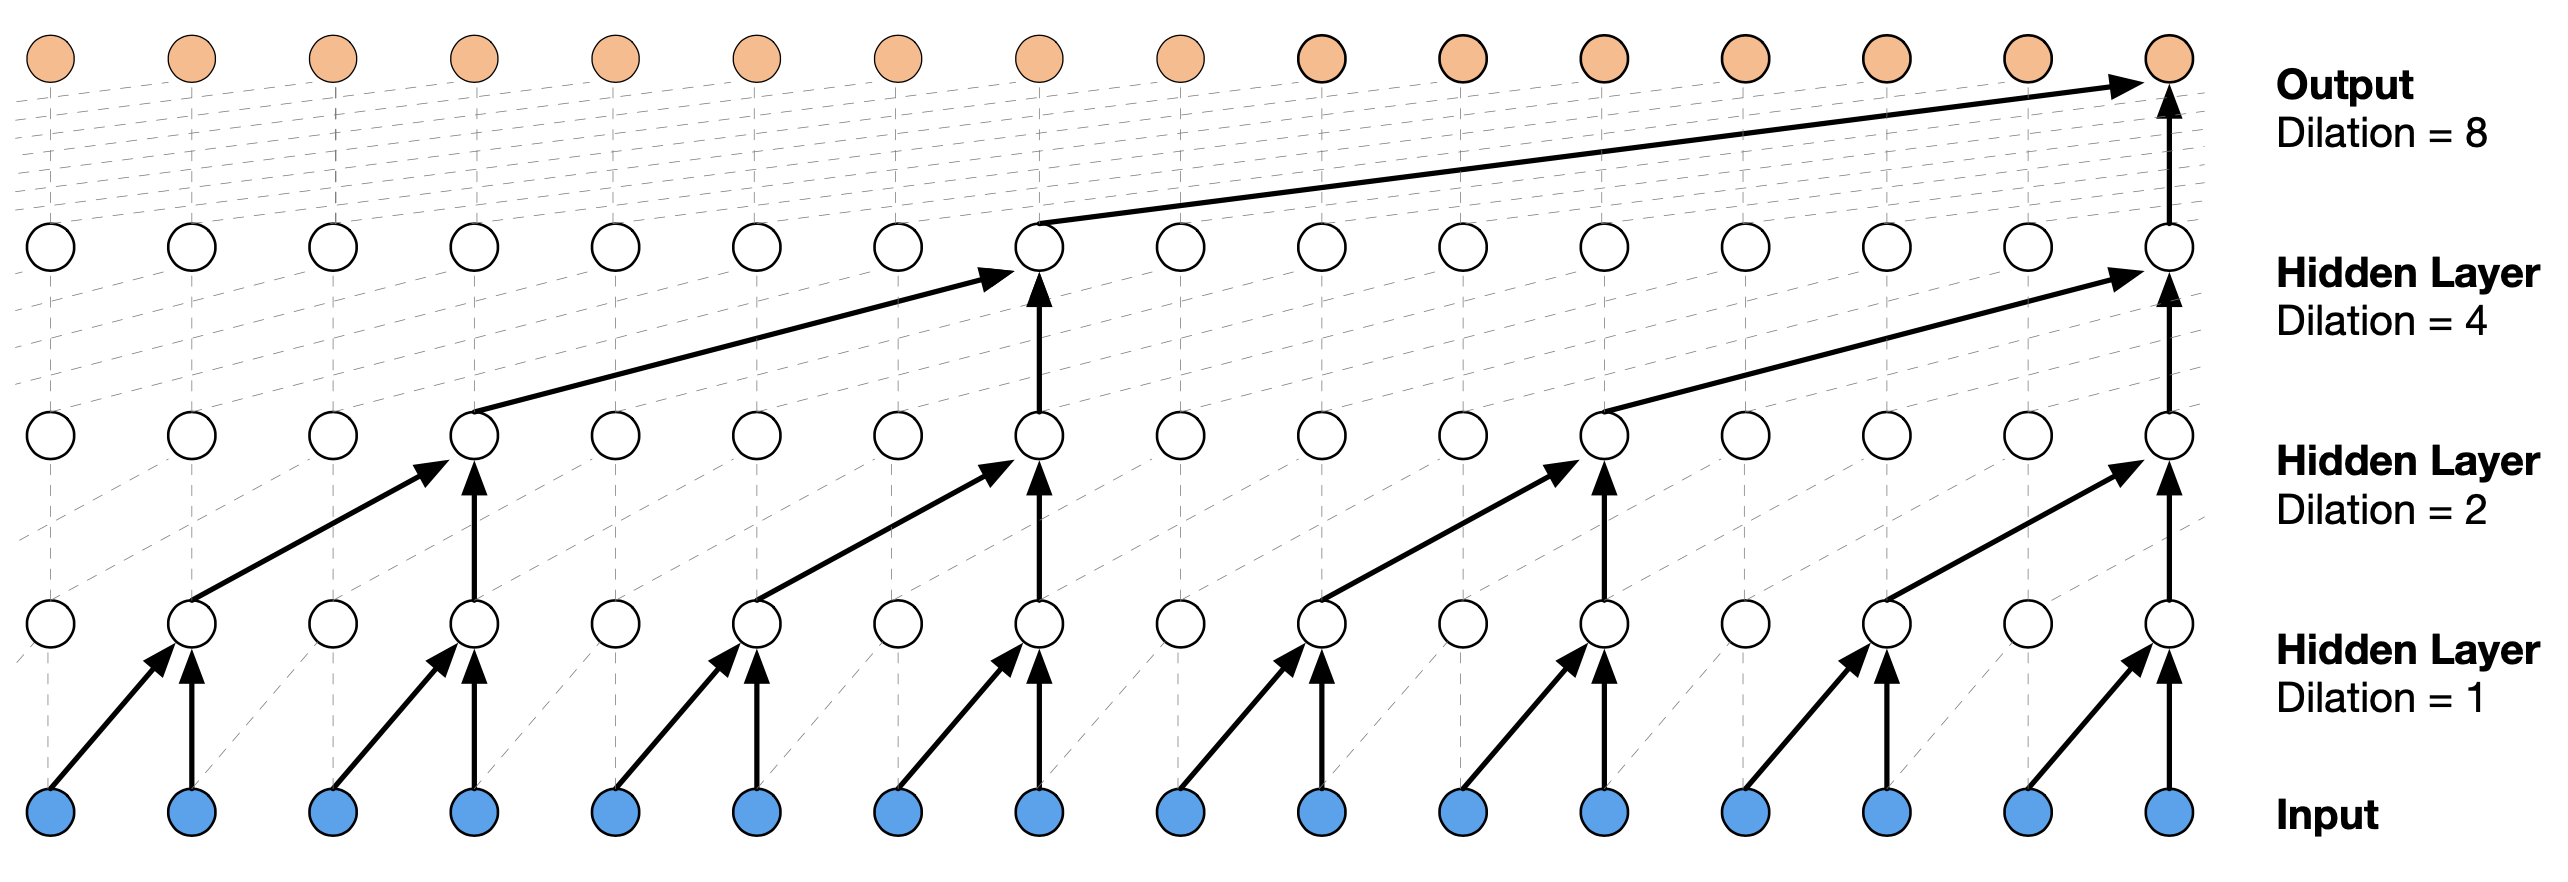
\includegraphics[width=0.95\textwidth]{figures/wavenet-dilated-causal-conv.png}
        \end{center}
        \caption{The Dilated Causal Convolution in WaveNet} 
        \label{fig:wavenet-dilated-causal-conv}
    \end{small}
\end{figure}



\paragraph{Gated Activation Units}
Each Convolution layer, Insteadof \textit{just} having a filter weight, also has a \textbf{gating weight}.
Hence the weights \(\mathbf{W} \in \mathbb{R}^{K \times 2} \), with \(K\) as the number of layers. 
The operation of layer $k \in [0, K]$, is parametrized as: 

\begin{equation}
    \mathbf{z} = \tanh ( \mathbf{x} * W_{k, f} ) \odot \sigma ( \mathbf{x} * W_{k, g} )
    \label{eq:wavenet-gated-activation}
\end{equation}





\paragraph{Summary of architechture}
The architecture is summed up in \cref{fig:wavenet-architecture}.
It's important to note that the Causal Convolution setup as described in \cref{fig:wavenet-dilated-causal-conv} only is applied \textit{once}, as the first layer.
This makes the entire rest of the network a simple convolutional network with dilation, as the \textbf{first (causal) convolutional stack ensures that the rest of the network will only see samples from the past.}
In all other respects we can consider this a standard CNN architecture. 


\begin{figure}
    \begin{small}
        \begin{center}
            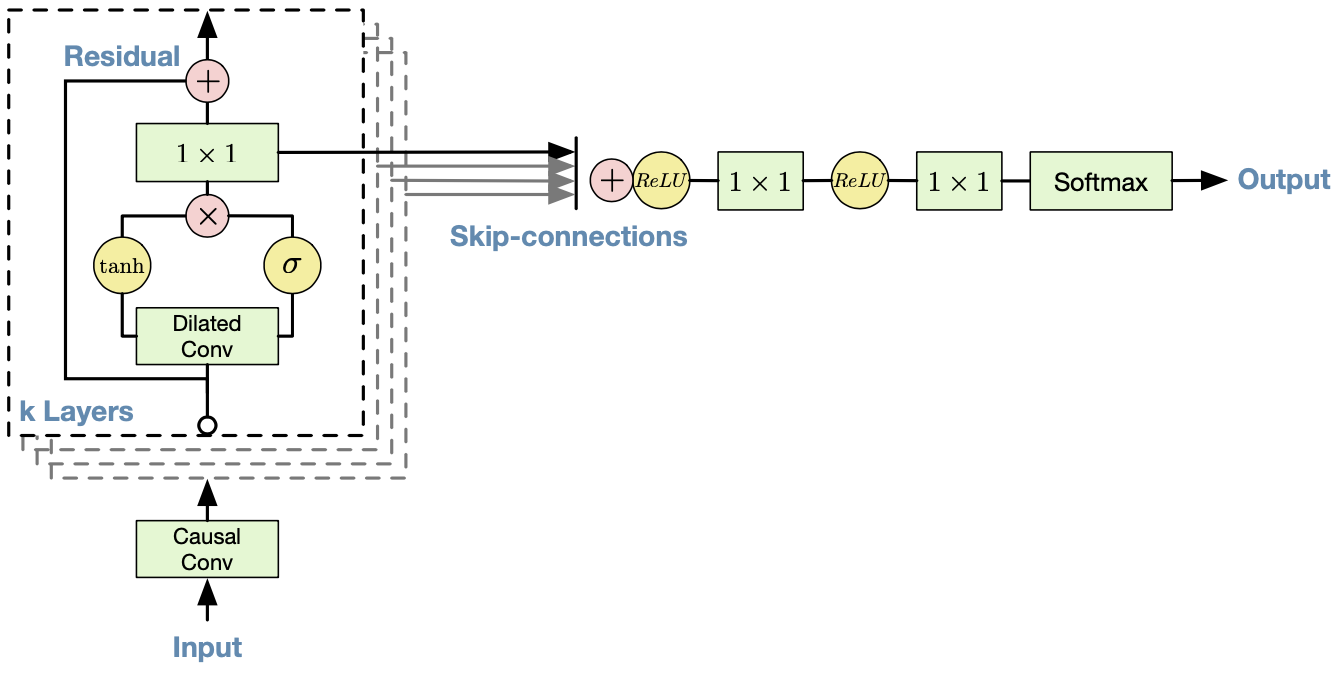
\includegraphics[width=0.95\textwidth]{figures/wavenet-architecture.png}
        \end{center}
        \caption{Overall Residual Architecture of WaveNet. 
        Skip connections happen from \textit{every Convolutional Layer} to the final softmax.}
        \label{fig:wavenet-architecture}
    \end{small}
\end{figure}


\subsubsection{Extending architecture to include latent representations of speaker}
It's possible to add a latent representation \(\mathbf{h}\), extending \cref{eq:wavenet-probabilities} to:

\begin{equation}\label{eq:wavenet-probabilities-ext}
    p(\mathbf{x}|\mathbf{h}) = \prod_{t=1}^T  p(x_t | x_1, ..., x_t, \mathbf{h} )
\end{equation}

There are two ways to represent this:

\paragraph{Global Conditioning (Speaker, Accent, Noise level)}
Here we set \(\mathbf{h}\) to a single global latent, representing a constant over the entire sequence. 
The activation from \cref{eq:wavenet-gated-activation} then becomes

\begin{equation}
    \mathbf{z} = \tanh ( \mathbf{x} * W_{k, f} + V^T_{k, f}\mathbf{h}) \odot \sigma ( \mathbf{x} * W_{k, g} + V^T_{k, g}\mathbf{h})
\end{equation}
With \(V_{k, *}\) is a linear projection , and the resulting vector \(V^T_{k, f}\mathbf{h}\) is broadcast over time \(T\).


\paragraph{Local Conditioning (Tone of voice, changing noise levels over the call}
Here we define \(h_t\), and use a ConvNet to upsample \(h_t\) to \(\mathbf{y} = f(\mathbf{h})\), so \cref{eq:wavenet-gated-activation} becomes:

\begin{equation}
    \mathbf{z} = \tanh ( \mathbf{x} * W_{k, f} + V_{k, f}*\mathbf{y}) \odot \sigma ( \mathbf{x} * W_{k, g} + V_{k, g}*\mathbf{y})
\end{equation}

\subsection{Results}

The main results here are evaluated on "subjective naturalness" by human evaluators. 
As such, WaveNets have outperformed previos TTS methods.
That's not really that interesting but it makes for a cool listen: \href{https://deepmind.com/blog/article/wavenet-generative-model-raw-audio}{here}

\newpage
\section{Vector Quantized VAE (VQ-VAE)}
Title:  \textit{Neural Discrete Representation Learning} \cite{oord_neural_2018}.
\\



Main points: 
\begin{itemize}
    \item Avoiding Posterior Collapse
    \item Discrete Latent
    \item With the right prior, generates speech/audio well  % TODO: elaborat
    \item Language Learning through raw speech
    \item Speaker Conversion
\end{itemize}


The main point of the VQ-VAE lies in that it uses a discrete (i.e. \textit{categorical}) embedding space as its latent space. 


\subsection{Model Components and Architecture}
The model is described in \cref{fig:vqvae-arch}.
What's very important to realize is that \textbf{the VQ-VAE is deterministic, not stochastic!}

\subsection{Discrete Latent Embedding Space}
The VQ VAE uses a \(D\)-dimensional latent space with \(K\) embedding vectors.
This means that the latent space \textbf{does not sample from a latent space} (so it's not a real VAE) but instead \textbf{does a nearest-neighbor embedding lookup}. 
We define the embedding vectors as 
\[
  e_i \in \mathbb{R}^D, i \in \{1 .. K\}, \therefore e \in \mathbb{R}^{K \times D}
\]

\begin{figure}[ht]
    \begin{small}
        \begin{center}
            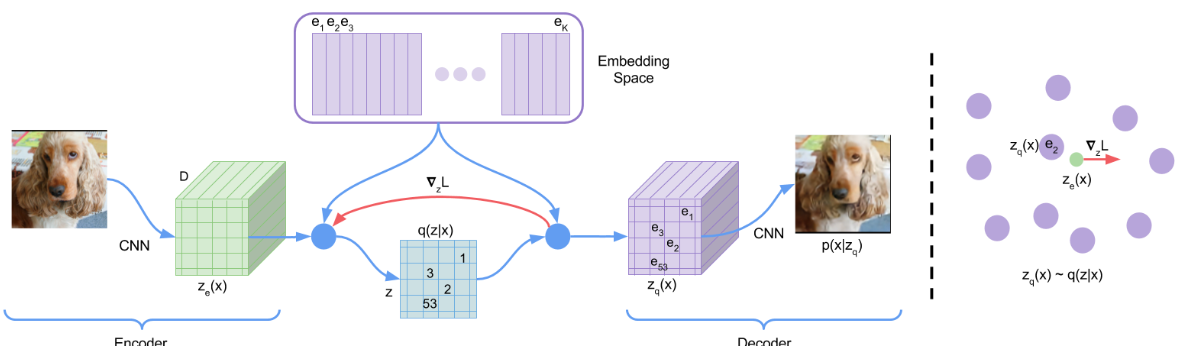
\includegraphics[width=0.95\textwidth]{figures/vqvae-arch}
        \end{center}
        \caption{VQ-VAE Architecture. 
        Right: Embedding space. 
        Left: Overall Architecture. 
        Note that the CNN works as a down/upsampling CNN, so as to avoid identity operations all the way through. 
        }
        \label{fig:vqvae-arch}
    \end{small}
\end{figure}

\subsection{Loss function}

The loss function \cref{eq:vqvae-loss} is composed of 3 parts, here covered in detail:

\begin{equation}
    L = 
    \log p(x| z_q(x)) + 
    || \mathrm{sg}[z_e (x) ] - e ||_2^2 + 
    || z_e (x)  - \mathrm{sg}[e] ||_2^2
    \label{eq:vqvae-loss}
\end{equation}

We denote \(z_e(x)\) as the \textbf{encoder output} and \(z_q(x)\) as the \textbf{quantized encoding.} 
We also use \(\mathrm{sg}\) to denote the stopgradient operator (identity function forward but 0 partial derivatives).

\paragraph{Reconstruction Loss}
\[
    \log p(x| z_q(x)) +     
\]
This refers to the probability of the data \(x\) given the embedding \(z_q(x)\).

The reconstruction loss is optimized by the \textbf{encoder} and \textbf{decoder}.

\paragraph{Embedding Loss}
\[
    || \mathrm{sg}[z_e (x) ] - e ||_2^2 
\]

The embedding loss quantifies \textit{how far away from the samples the embeddings are.}
This loss comes from Vector Quantization (VQ), a dictionary learning algorithm. 
The VQ objective seen here moves the \textit{discretized} embedding vectors \(e_i \in \mathbb{R}^D\) towards the \textit{continuous encoder outputs} \(z_e(x)\).
This means that the model is able to learn embeddings and update them at need. 

The embedding loss is optimized by the \textbf{embedding}.

\paragraph{Commitment Loss}
\[
    || z_e (x)  - \mathrm{sg}[e] ||_2^2
\]
The commitment loss quantifies \textit{how far away from the embeddings a sample is.}
The embedding space is dimensionless in volume, and therefore the output of the encoder can grow arbitrarily large, while embeddings can't keep up. 
This equates to the encoder seeing an out-of-distribution sample and encoding it as very far away from the latent space embeddings. 

The commitment loss is optimized by the \textbf{encoder}.



\subsection{Experiments and Results}

\subsubsection{Images}
Downsampling from \(128 \times 128 \times 3 \) to a \( 32 \times 32 \times 1 \) discretized latent space on the ImageNet ( \(128 \times 128 \times 3\) ) dataset.

For images, the encoder/decoder is the PixelCNN. 



\subsubsection{Audio}
For audio, the VQ-VAE is trained on the VCTK dataset, which has 109 different speakers. 
The encoder is \textbf{6 strided convolutions with stride 2 and window-size 4}, corresponding to a downsampling of 64x. 
The latent space is a single 512-dimensional discretized space. 
In addition to the latent space, the decoder is conditioned on a 1-hot speaker embedding. 

In order to make a prior for the latent space distribution, the authors trained a WaveNet model on the latent variables and used it as a prior on the latent space. \cite{oord_wavenet_2016}


\paragraph{Results}
The VQ-VAE manages to learn to interchange speakers very well. To cite the paper:

\begin{displayquote}
    This means that the VQ-VAE has, without any form of linguistic supervision, 
    learned a high-level abstract space that is invariant to low-level features and only encodes the content of the speech.
\end{displayquote}


The authors also ran an experiment where they mapped a 128-dimensional discrete latent space to 41 phonemes. 
Using this simple mapping they found the accuracy to be \(49.3\%\), without further mappings. 



\newpage
\section{Clockwork Variational Autoencoders}
\paragraph{Authors} Vaibhav Saxena, Jimmy Ba, Danijar Hafner. \cite{saxena_clockwork_2021}

The clockwork VAE aims to learn higher-level, abstract prediction timelines \textit{without needing to predict the actual images going forward.}
They term this "Temporally Abstract Latent Dynamics Models".


\subsection{CW-VAE Architecture and components}
The CW-VAE is composed of a hierarchy of "states" as seen in \cref{fig:cwvae-architecture}

\begin{figure}[hb]
    \begin{small}
        \begin{center}
            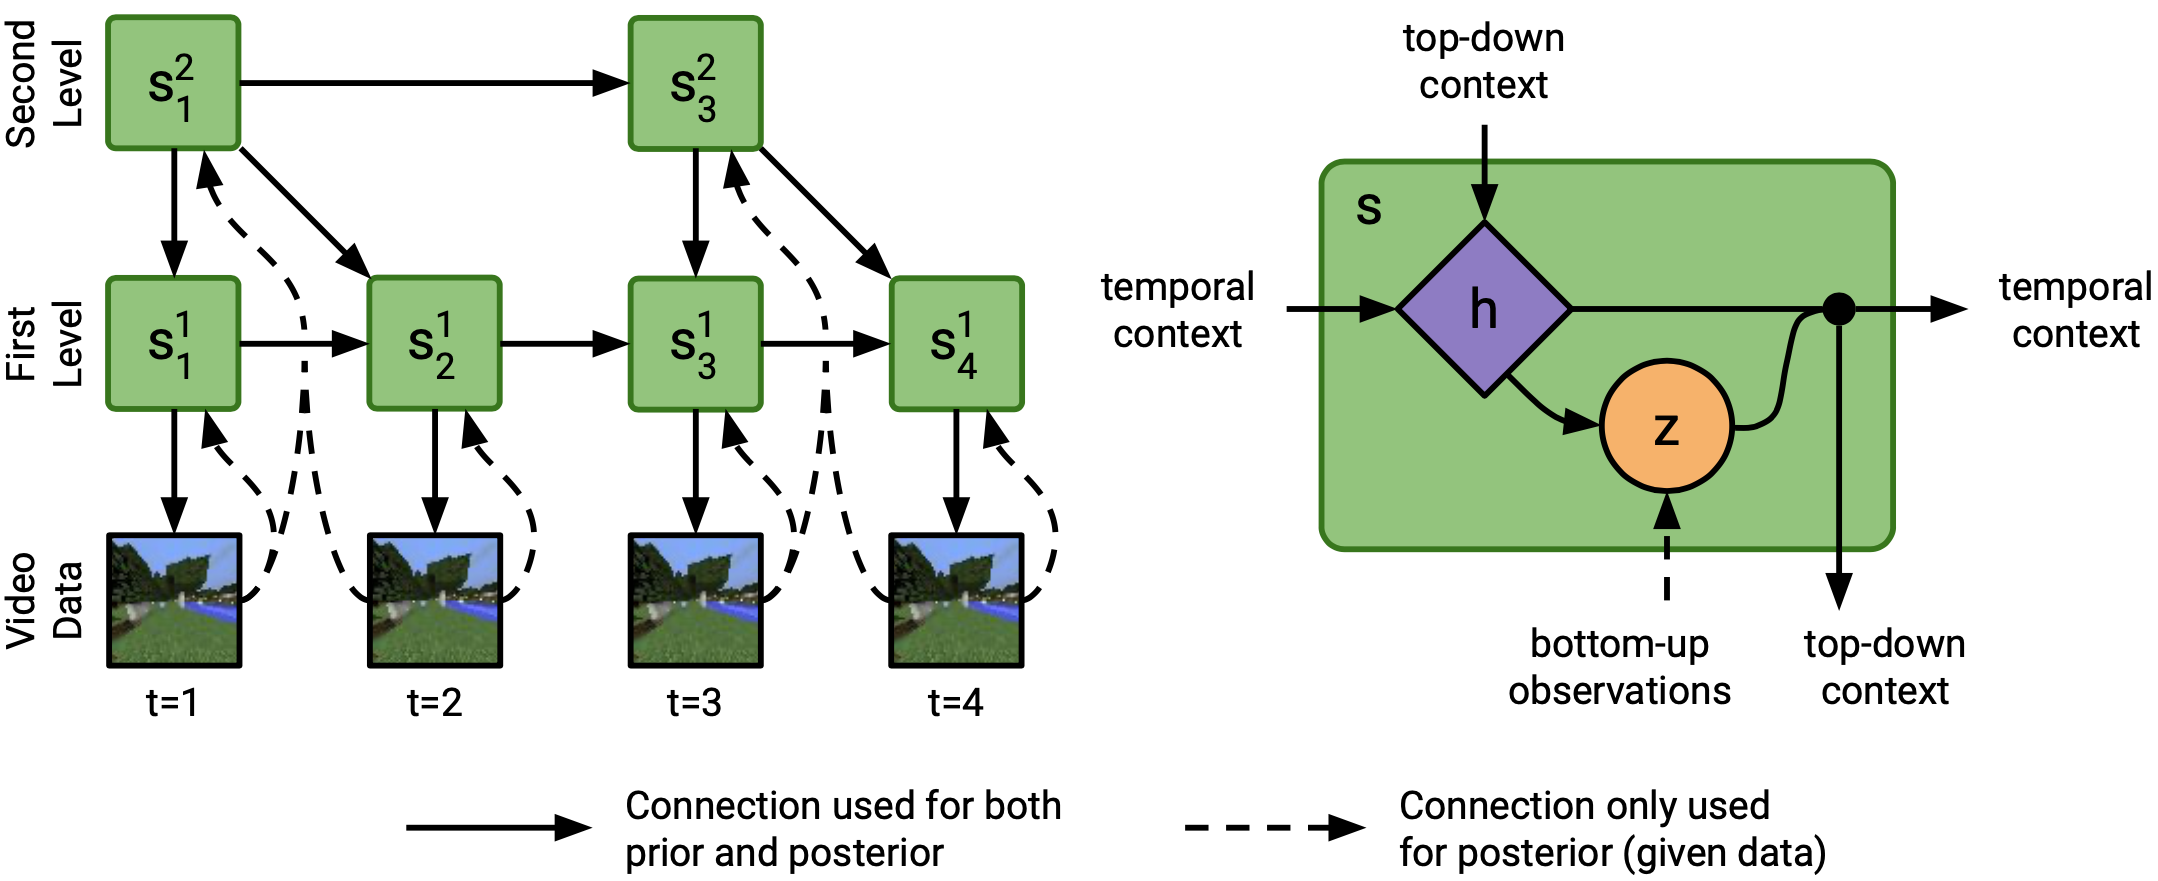
\includegraphics[width=0.95\textwidth]{figures/cwvae-architecture.png}
        \end{center}
        \caption{
            \textbf{Arrows:} Solid is the generative model, dashed is the inference model. 
            \textbf{Left:} The general setup of the CW-VAE, with a temporal abstraction factor \(k=2\). 
            The upper state only updates every kth timestep, and this would compound in higher hierarchies. 
            As such we see that the video frame with \(t=2\) still will feed into \(s^2_1\), and likewise the frame at \(t=4\) feeds into \(s^2_3\)
            \textbf{Right:} The internals of states \(s_l^t\). 
            }
        \label{fig:cwvae-architecture}
    \end{small}
\end{figure}

\subsubsection{The latent states \(s^l_t\)}

The latent state is composed of a deterministic variable \(h_t\) and a stochastic variable \(z_t\). 


\paragraph{Updates to latent states during inference}
The latent states are updated at the "active" timesteps 
\(\mathcal{T}_l = \{ t \in [1, T] | t \mathrm{mod} k^{l-1} = 1 \}\), 
where \(k\) is the dilation factor.
This means that latent states will only be updated at each \(k_{l-1}\) timestep, where \(l\) is the "level" of the latent variable.
Otherwise, the states are copied from the previous timestep.

During inference, all "active" latents will receive a CNN image embedding (in \cref{fig:cwvae-architecture} this is the "bottom-up observations").
The posterior \(q^l_t\) for that latent is calculated 
"as a function (what function?) of the input features, 
\hl{(ASK JAKOB: Is this the arrow from $z$ to the combination node?) } 
the posterior sample at the previous step (temporal context), 
and the posterior sample above (top-down context)"
The posterior / "Gaussian Belief" \(q^l_t\), which is a diagonal Gaussians with means and variances predicted from the deterministic variable.


The deteministic variable is updated with a GRU at every active step.

\subsubsection{Embeddings and layers in between.}

The authors (Appendix C) claim to have used "architectures very similar to the DCGAN".

The DCGAN paper's decoder architecture is shown in \cref{fig:cwvae-dcgan-arch}. \cite{radford_unsupervised_2016}

\begin{figure}[hb]
    \begin{small}
        \begin{center}
            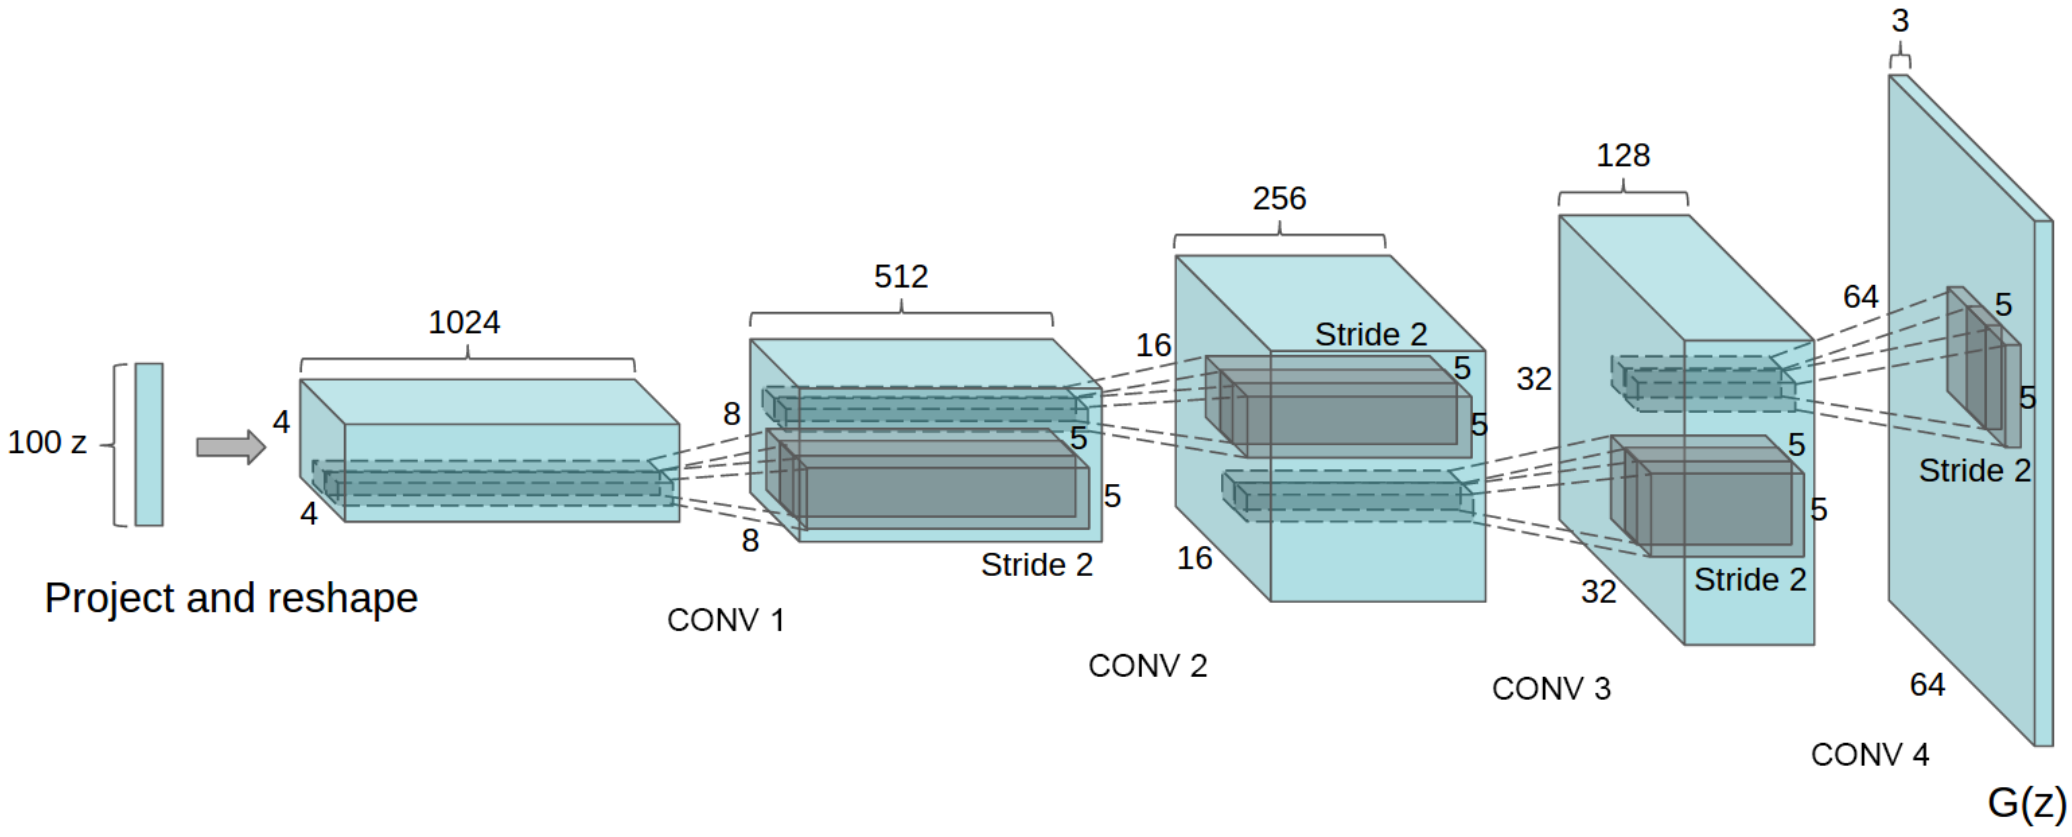
\includegraphics[width=0.95\textwidth]{figures/cwvae-dcgan-arch.png}
        \end{center}
        \caption{\textit{From DCGAN paper: }
        A 100 dimensional uniform distribution Z is projected to a small spatial extent convolutional representation with many feature maps.
        A series of four fractionally-strided convolutions (in some recent papers, these are wrongly called
        deconvolutions) then convert this high level representation into a 64 × 64 pixel image. Notably, no
        fully connected or pooling layers are used.}
        \label{fig:cwvae-dcgan-arch}
    \end{small}
\end{figure}



\subsection{General Comments} % (fold)
The CWVAE paper manages to show very promising results in terms of temporal abstraction. 
They also conjecture that they would be able to do similar things with "more data more GPU" but that we lack good validation metrics. 


NB This paper has a good appendix to keep in mind. 

% subsection General Comments (end)


\newpage
\section{Hierarchical Multiscale Recurrent Neural Networks}
\paragraph{Authors}: Junyoung Chung, Sungjin Ahn, Yoshua Bengio \cite{chung_hierarchical_2017} \\

\begin{figure}[ht!]
    \begin{small}
        \begin{center}
            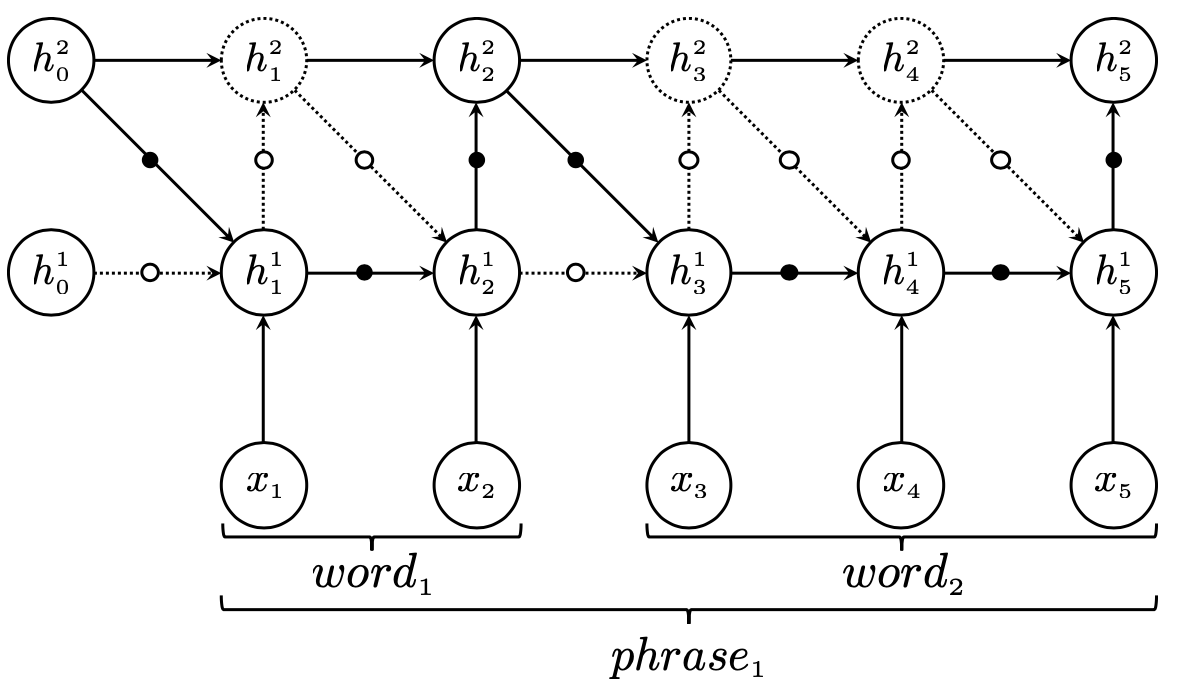
\includegraphics[width=0.55\textwidth]{figures/hmrnn-architecture.png}
        \end{center}
        \caption{Overall Architecture of HMRNN. 
        HM-RNN should learn and discover the structure of the data by itself, textbf{without the use of boundary tokens}. 
        }
        \label{fig:hmrnn-architecture}
    \end{small}
\end{figure}


\subsection{Problem}
The HMRNN addresses the question:
\begin{quote}
    Can an RNN discover hierarchical multiscale structure without explicit hierarchical boundary information?
\end{quote}


\paragraph{Temporal-hierarchical information learning}
Temporal-Hierarchical information exist in many kinds of sequential data, and can easily be explained as a hierarchy of character, word, sentence, and paragraph context. 

\paragraph{Unsupervised boundary detection}
The authors see the unsupervised boundary objective as necessary to learn a temporal-hierarchical information representation from data.
In the past, there have been attempts at setting up a hierarchy of RNNs with the time hierarchies as hyperparameters, 
but allowing the model to learn this unsupervised has advantages:
\begin{enumerate}
    \item The model is robust to variable length words/sentences. 
    \textit{Example:} \texttt{hello} and \texttt{hi} \textit{contain roughly the same word-level information, 
    although one is almost 3 times as long as the other.}
    \item When progressing past a word and sentence-level abstraction, the ground truth information available quickly decreases.
    \textit{Example: Line breaks, paragraph breaks, hyphens, and chapter breaks are very sparsely represented in text datasets.}
\end{enumerate}




\subsection{HMRNN model and components}
The model is summarized in \cref{fig:hmrnn-architecture}.

The HMRNN Model includes a binary boundary detector at each layer, which triggers the different operations. 

\paragraph{COPY, FLUSH, and UPDATE operations} in the HM-RNN are implemented at each abstraction level.

\begin{itemize}
    \item COPY operation copies the state of the current abstraction level to the next cell
    \item UPDATE sparsely nupdates the cell in the next level 
    \item FLUSH happens when a boundary is detected, 
    so the current state representation is ejected to the higher level cell, and the state is reinitialized.
\end{itemize}


\paragraph{Boundary detection gradients and the Slope Annealing Trick} are used with the straight-through estimator, to account for the non-differentiability of the discrete variable. 
Hence, during the backwards pass, the step function used in the forward pass is replaces with a hard sigmoid.
The Slope Annealing trick includes starting the slope of the hard sigmoid as $a=1$ and increasing it during training for the network to slowly learn to pass information through the sigmoid. 


\paragraph{The HM-LSTM} is proposed, as an LSTM model with \(l\in[0...L]\), performing the following update at step $t$ for layer $l$
\begin{equation}\label{eq:hmlstm-update}
     \mathbf{h}^l_t, \mathbf{c}^l_t, z^l_t =
    f^l_{HM-LSTM}(
        \mathbf{c}^l_{t-1}, 
        \mathbf{h}^l_{t-1}, \mathbf{h}^{l-1}_{t}, \mathbf{h}^{l+1}_{t-1},
        z^l_{t-1}, z^{l-t}_t
        )
\end{equation}
with \(f^l_{HM_LSTM}\) being implemented s.t.


\begin{figure}
    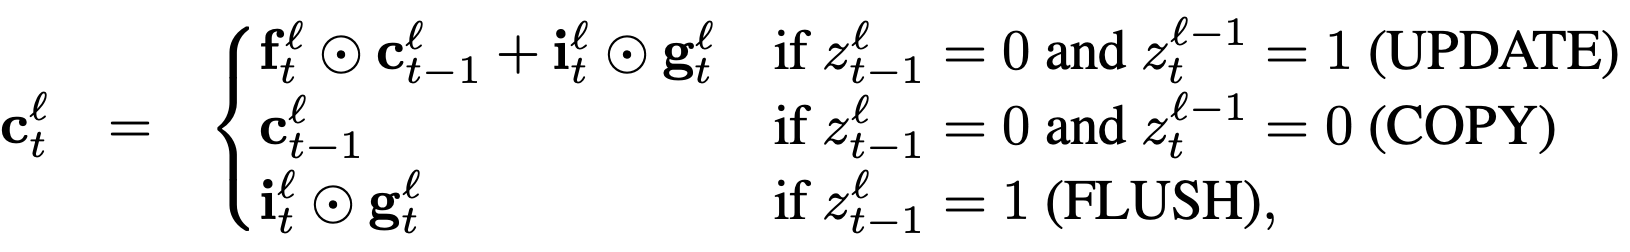
\includegraphics[width=0.45\textwidth]{figures/hmlstm-cell.png}
    \caption{
        HM-LSTM cell state update.
        Here $(f,i,o)$ are gates (forget, input, output) and $g$ is a proposal vector for the cell state.
        }
    \label{eq:hmlstm-cell}
\end{figure}



\paragraph{Model setup for experiments} have the following:
\begin{enumerate}
    \item A continuous input embedding layer
    \item HM-LSTM recurrent unit (3 layers for CL-LM)
    \item Output module of a FFNN, an output embedding layer and a softmax for probability calculation
\end{enumerate}
Here the output module will receive the hidden states of all RNN layers as inputs, adding a gating layer
\begin{equation}
    g^l_t = \mathtt{sigm}(\mathbf{w}^l, [\mathbf{h}^1_t ... \mathbf{h}^L_t])
    \label{eq:hmlstm-output-gate}
\end{equation}
And an output embedding as
\begin{equation}
    \mathbf{h}^e_t = \mathtt{ReLu}
    \left( 
        \sum_{l=1}^L 
        g^l_t
        W^l_t
        \mathbf{h}^l_t   
     \right)
    \label{eq:hmlstm-output-embedding}
\end{equation}



\subsection{Experiments and results}

\paragraph{Character-level language modelling} providing raw text as input, is an ideal task for evaluating raw boundary detection. 
They train the CLLM task using the NLL sequence objective: 
\begin{equation}
    \min_\theta - \frac{1}{N}\sum^N_{n=1}\sum_{t=1}^{T^n} \log p(x^n_t | x^n_{<t}, \theta)
    \label{eq:hmlstm-nll}
\end{equation}

The results on boundary detection are shown in \cref{fig:hmlstm-fun}


\begin{figure}
    \begin{small}
        \begin{center}
            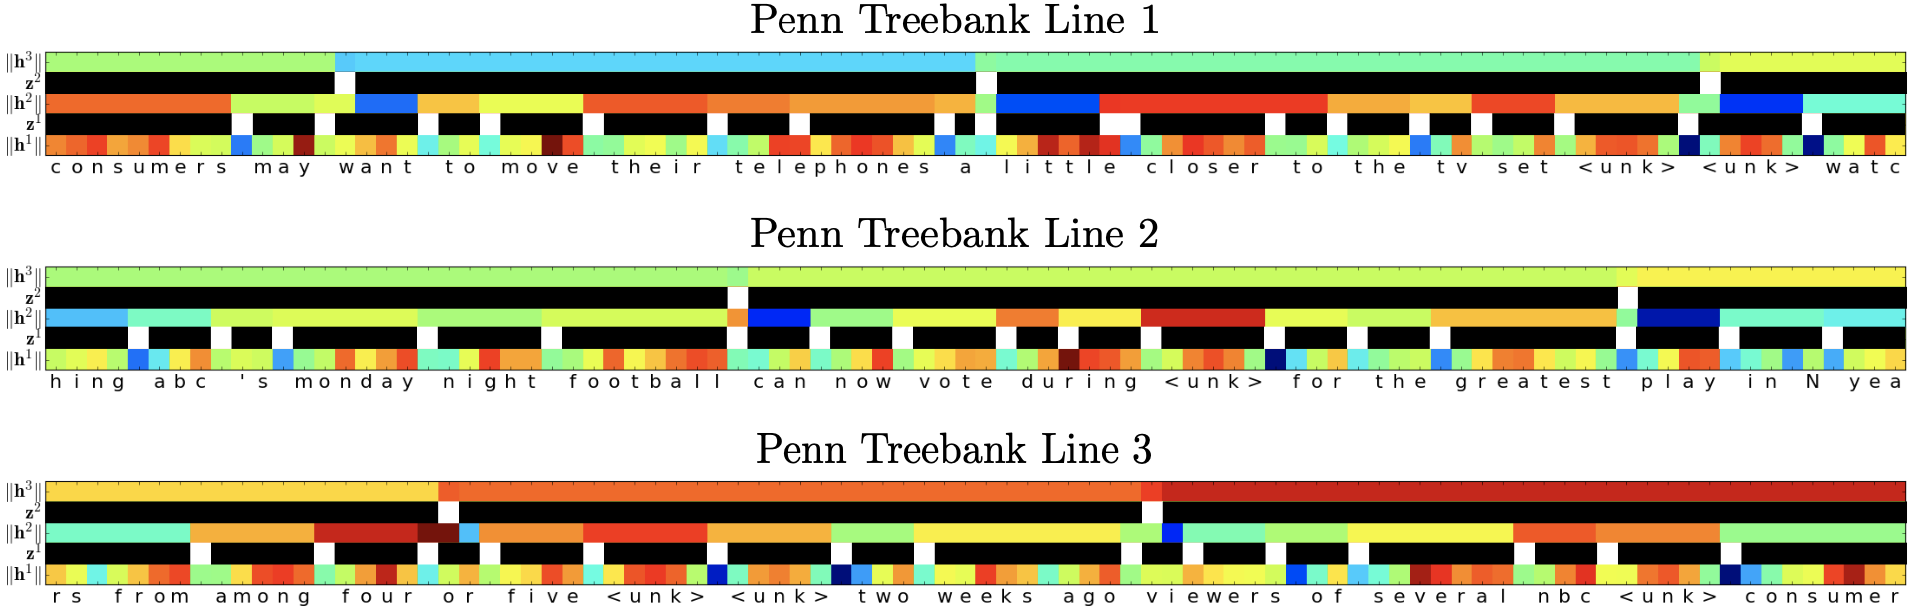
\includegraphics[width=0.95\textwidth]{figures/hmlstm-states.png}
        \end{center}
        \caption{$l^2$ norm of hidden states along with boundary detection states for PTB.l}
        \label{fig:hmlstm-states}
    \end{small}
\end{figure}





\newpage


\section{Variational Temporal Abstraction}\label{sec:VTA}
\paragraph{Authors}: Taesup Kim, Sungjin Ahn, Yoshua Bengio \cite{kim_variational_2019} \\



\paragraph{Overview} % (fold)
\label{par:Overview}
This paper is among the first to combine two recurrent state space model with latent variables. 

They frame the problem as a temporal imaginative structure that should be probed, and reference the HMRNN model as a good first step.
The entire point of the paper is trying to find an "imaginative" model that can also use the latent stochastic variables to model future possibilities. 



% paragraph Overview (end)

\subsection{Model} % (fold)
\label{sub:VTA-Model}

Given a sequence \(X = x_{1:T} \) we can split it into subsequences \(X = (X_1, \dots , X_N) \) with lengths \(L={l_i}\) such that \(T=\sum^N_{i=1}l_i\). 
The VTA authors split the subsequences based on $N$ and $L$ as \textit{discrete latent variables}. 

Furthermore, they introduce the terms \textit{temporal abstraction} $z_i$ which generates $X_i$ and an \textit{observation abstraction} $s_t$ which generates observation $x_t$.
As such, an observation $x_t\in X_i$ depends on both $z_i$ and $s_t$, while the transitions of each level happen at subsequence scale for $z_i$ and at each time step for $s_t$. 

The joint generative model can be written as:

\begin{equation}
    p(X,S,L,Z,N) = p(N)
    \prod_{i=1}^N
    p(X_i,S_i|z_i, l_i)
    p(l_i|z_i)
    p(z_i|z_{<i})
    \label{eq:vta-generative}
\end{equation}
With the subsequence joint distribution:
\begin{equation}
    p(X_i,S_i|z_i,l_i) = 
    \prod^{l_i}_{j=1}
    p(x^i_j|s^i_j)
    p(s^i_j|s^i_{<j}, z_i)
    \label{eq:vta-subseq-joint}
\end{equation}

The authors argue that even if it is possible to use a Markovian SSM or HMM in \cref{eq:vta-generative} and \cref{eq:vta-subseq-joint}, using a RSSM type approach solves this better. 
This is because the RSSM includes a deterministic RNN path which can encode complex long-term dependencies within the model, which is a weakness of HMM type models. 

% subsection Model (end)


\newpage
\section{A Clockwork RNN}
\paragraph{Authors}: Jan Koutník, Klaus Greff, Faustino Gomez, Jürgen Schmidhuber \cite{koutnik_clockwork_2014} \\



\newpage
\section{Towards Generating Long and Coherent Text with Multi-Level Latent Variable Models }
\paragraph{Authors} Dinghan Shen, Asli Celikyilmaz, Yizhe Zhang, Liqun Chen, Xin Wang, Jianfeng Gao, Lawrence Carin \cite{shen_towards_2019} \\



\newpage
\section{Transformer-XL: Attentive Language Models Beyond a Fixed-Length Context}
\paragraph{Authors} Zihang Dai, Zhilin Yang, Yiming Yang, Jaime Carbonell, Quoc V. Le, Ruslan Salakhutdinov % \cite{shen_towards_2019} \\



\newpage
\section{TacoTron}
\paragraph{Authors:} Yuxuan Wang,\dots , Rob Clark, Rif A. Saurous \cite{wang_tacotron_2017}


\subsection{Problem to solve}
End2End Text-To-Speech is a remaining frontier for ML systems, typically requiring extensive in-subject technical knowledge to set up. 
The goal of a end2end TTS system that can model \(p(\mathtt{Audio}|\mathtt{Text})\) directly, is therefore very useful. 
The main issue here, is that TTS encompasses an \textit{Inverse Problem}, i.e. a problem where the input dimensionality is much LOWER than the output dimensionality. 

Tacotron is proposed as an integrated end-to-end generative TTS model that takes a character sequence as input and outputs the corresponding spectrogram. 

\subsection{Architecture}
\begin{figure}[h!]
    \centering
    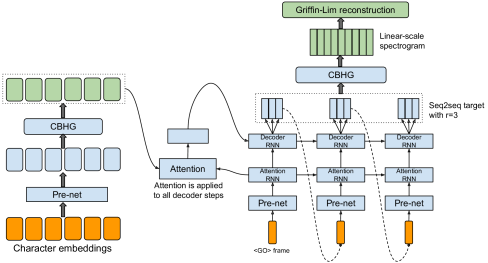
\includegraphics[width=\textwidth]{figures/tacotron-arch.png}
    \caption{Overall architecture of TacoTron TTS system. 
    The CBHG module is described in \cref{fig:tacotron-cbhg}}
    \label{fig:tacotron-arch}
\end{figure}


\paragraph{Convolution Bank + Highway Net + Bidirectional GRU feature}
(CBHG) consists of a bank of 1-D convolutional filters, followed by highway networks and a bidirectional gated recurrent unit (GRU). 
The input sequence is first convolved with 
\(K\) sets of 1-D convolutional filters, where the $k$-th set contains $C_k$ filters, like modelling unigrams, bigrams, \dots $K$-grams.  

Convolution outputs are fed into a multi-layer highway network to extract high-level features. 
Finally, we stack a bidirectional GRU RNN on top to extract sequential features from both forward and backward context.

See \cref{fig:tacotron-cbhg} for a visual.

\begin{figure}[h!]
    \centering
    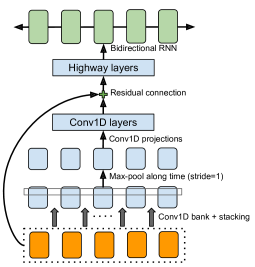
\includegraphics[width=0.55\textwidth]{figures/tacotron-cbhg.png}
    \caption{The CBHG module in the TacoTron architecture. }
    \label{fig:tacotron-cbhg}
\end{figure}

\paragraph{The Encoder} 
on the left side of \cref{fig:tacotron-arch} passes the input character embedding sequence 
to a bottleneck layer and through a CBHG to an encoded representation of the entire sequence.  


\paragraph{The Decoder} consists of a 2-layer FC pre-net, an Attention GRU (RNN), and a Decoder stack of GRUs with vertical residual connections. 




\newpage
\bibliographystyle{abbrv}
\bibliography{vseq}

\end{document}
